\documentclass{article}

\usepackage{polski}
\usepackage{amsmath}
\usepackage{graphicx}
\usepackage{float}
\usepackage{subfig}
\usepackage{multirow}
\usepackage{chngpage}

\title{Aproksymacja średniokwadratowa wielomianami trygonometrycznymi}
\author{\textbf{Łukasz Wala}\\
    \textit{AGH, Wydział Informatyki, Elektroniki i Telekomunikacji} \\
    \textit{Metody Obliczeniowe w Nauce i Technice 2021/2022}}
\date{Kraków, \today}

\begin{document}
\maketitle

\section{Opis problemu}
Główną ideą zadania jest zbadanie zachowania funkcji przybliżonej za pomocą aproksymacji
średniokwadratowej wielomianami trygonometrycznymi.

Badana funkcja:
\[f(x)=x^2-m\cdot\cos\left(\frac{\pi x}{k}\right)\]
Gdzie $k=\frac{1}{2}$, $m=4$ oraz $x\in [-6,6]$.

\section{Opracowanie}
\subsection{Wyprowadzenie}
W aproksymacji średniokwadratowej poszukiwana jest wartość minimalna sumy kwadratów różnic funkcji aproksymowanej $F(x)$
oraz funkcji aproksymującej $f(x)$ z uwzględnieniem funkcji wagowej $w(x)$ większej od zera (tutaj $\forall x \in D
:w(x) = 1$). Funkcją aproksymującą ma być wielomian trygonometrycznym o postaci
$$\displaystyle f(x) = a_0 + \sum_{j=1}^mb_j\cos(jx)\:+\:\sum_{j=1}^m a_j\sin(jx)$$

Więc błąd średniokwadratowy przyjmuje postać

$$\displaystyle H(a_0, ..., a_m, b_1, ..., b_m)=\sum_{i=1}^nw(x_i)\left[F(x_i)-(a_0 + \sum_{j=1}^mb_j\cos(jx_i)\:+\:\sum_{j=1}^m a_j\sin(jx_i))\right]^2$$

Aby funkcja przyjmowała wartość minimalną względem współczynnka $c$, pochodna funkcji względem tego współczynnika musi
wynosić zero

$$\frac{\partial H}{\partial c}=0, c \in \{a_0, ..., a_m, b_1, ..., b_m\}$$

Na przykład dla $a_k$

$$\displaystyle -2\sum_{i=1}^nw(x_i)\left[F(x_i)-(a_0 + \sum_{j=1}^mb_j\sin(jx_i)\:+\:\sum_{j=1}^m a_j\cos(jx_i))\right]\cos(kx_i) = 0$$

Po przekształceniach dla $a_0$
\begin{multline*}
    $$\displaystyle \sum_{i=0}^nw(x_i)a_0+\sum_{j=1}^m\left(\sum_{i=0}^nw(x_i)\cos(jx_i)\right)a_j+
    \sum_{j=1}^m\left(\sum_{i=0}^nw(x_i)\sin(jx_i)\right)b_j \\=\sum_{i=0}^nw(x_i)F(x_i)$$
\end{multline*}

Dla $a_k, k\in\{1,2,...,m\}$:
\begin{multline*}
    $$\displaystyle \sum_{i=0}^nw(x_i)\cos(kx_i)a_0+\sum_{j=1}^m\left(\sum_{i=0}^nw(x_i)\cos(kx_i)\cos(jx_i)\right)a_j+
    \sum_{j=1}^m\left(\sum_{i=0}^nw(x_i)\cos(kx_i)\sin(jx_i)\right)b_j \\ =\sum_{i=0}^nw(x_i)F(x_i)\cos(kx_i)$$
\end{multline*}

Oraz dla $b_k, k\in\{1,2,...,m\}$
\begin{multline*}
    $$\displaystyle \sum_{i=0}^nw(x_i)\sin(kx_i)a_0+\sum_{j=1}^m\left(\sum_{i=0}^nw(x_i)\sin(kx_i)\cos(jx_i)\right)a_j+
    \sum_{j=1}^m\left(\sum_{i=0}^nw(x_i)\sin(kx_i)\sin(jx_i)\right)b_j \\ =\sum_{i=0}^nw(x_i)F(x_i)\sin(kx_i)$$
\end{multline*}

Z tych równań można zbudować układ
\[
\begin{bmatrix}
    \sum_{i=0}^nw(x_i) & \sum_{i=0}^nw(x_i)\cos(1\cdot x_i) & \sum_{i=0}^nw(x_i)\sin(1\cdot x_i) & \hdots \\
    \sum_{i=0}^nw(x_i)\cos(1\cdot x_i) & \sum_{i=0}^nw(x_i)\cos(1\cdot x_i)\cos(1\cdot x_i) & \sum_{i=0}^nw(x_i)\cos(1\cdot x_i)\sin(1\cdot x_i) & \hdots\\
    \sum_{i=0}^nw(x_i)\sin(1\cdot x_i) & \sum_{i=0}^nw(x_i)\sin(1\cdot x_i)\cos(1\cdot x_i) & \sum_{i=0}^nw(x_i)\sin(1\cdot x_i)\sin(1\cdot x_i) & \hdots\\
    \sum_{i=0}^nw(x_i)\cos(2\cdot x_i) & \sum_{i=0}^nw(x_i)\cos(2\cdot x_i)\cos(1\cdot x_i) & \sum_{i=0}^nw(x_i)\cos(2\cdot x_i)\sin(1\cdot x_i) & \hdots\\
    \sum_{i=0}^nw(x_i)\sin(2\cdot x_i) & \sum_{i=0}^nw(x_i)\sin(2\cdot x_i)\cos(1\cdot x_i) & \sum_{i=0}^nw(x_i)\sin(2\cdot x_i)\sin(1\cdot x_i) & \hdots\\
    \vdots & \vdots & \vdots & \vdots \\
    \sum_{i=0}^nw(x_i)\cos(m\cdot x_i) & \sum_{i=0}^nw(x_i)\cos(m\cdot x_i)\cos(1\cdot x_i) & \sum_{i=0}^nw(x_i)\cos(m\cdot x_i)\sin(1\cdot x_i) & \hdots\\
    \sum_{i=0}^nw(x_i)\sin(m\cdot x_i) & \sum_{i=0}^nw(x_i)\sin(m\cdot x_i)\cos(1\cdot x_i) & \sum_{i=0}^nw(x_i)\sin(m\cdot x_i)\sin(1\cdot x_i) & \hdots\\
\end{bmatrix}
\cdot
\]

\[
\cdot
\begin{bmatrix}
    a_0 \\
    a_1 \\
    b_1 \\
    a_2 \\
    b_2 \\
    \vdots \\
    a_m \\
    b_m \\ 
\end{bmatrix}
=
\begin{bmatrix}
    \sum_{i=0}^nw(x_i)F(x_i) \\
    \sum_{i=0}^nw(x_i)F(x_i)\cos(1\cdot x_i) \\
    \sum_{i=0}^nw(x_i)F(x_i)\sin(1\cdot x_i) \\
    \sum_{i=0}^nw(x_i)F(x_i)\cos(2\cdot x_i) \\
    \sum_{i=0}^nw(x_i)F(x_i)\sin(2\cdot x_i) \\
    \vdots \\
    \sum_{i=0}^nw(x_i)F(x_i)\cos(m\cdot x_i) \\ 
    \sum_{i=0}^nw(x_i)F(x_i)\sin(m\cdot x_i)
\end{bmatrix}    
\]

Również pod uwagę trzeba wziąć, że punkty z przedziału $[a,b]$ muszą być zawsze (podczas wyliczania wartości macieży oraz podczas wyliczania wartości
funkcji aproksymującej) mapowane na przedział $[0, 2\pi]$ za pomocą funkcji

$$c(x)=\frac{2\pi (x-a)}{b-a}$$

Do rozwiązania powyższego układu równań użyta została funkcja \textit{linalg.solve} z pakietu \textit{numpy}
w języku Python.

\subsection{Wykresy}
Pierwszym krokiem analizy będzie zbadanie zachowania wykresów funkcji aproksymujących. Zakres liczby punktów użytych do
stworzenia funkcj wynosi 7-50 z wykorzystaniem wielomianów stopni 3-30 (2 * stopień + 1 = liczba funkcji bazowych), przy 
zachowaniu założenia, że liczba węzłów musi być większa lub równa liczbie funkcji bazowych. Punkty rozłożone są
równomierne na przedziale.

\begin{figure}[H]
    \centering
    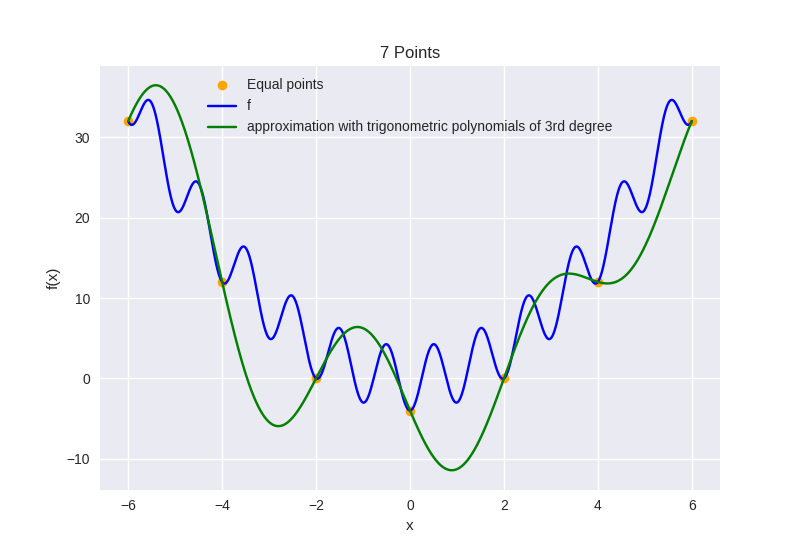
\includegraphics[width=\textwidth]{img/tripoly_3_7.png}
    \caption{Aproksymacja średniokwadratowa wielomianami trygonometrycznymi 3 stopnia}
\end{figure}

\begin{figure}[H]
    \centering
    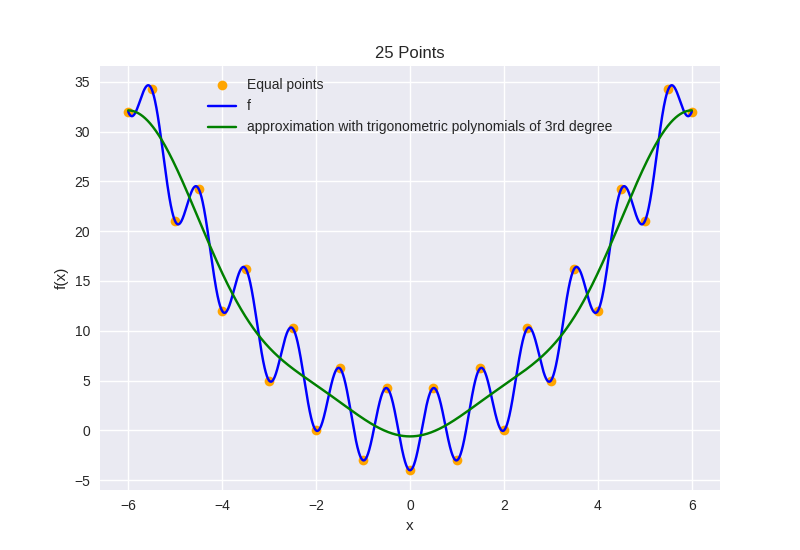
\includegraphics[width=\textwidth]{img/tripoly_3_25.png}
    \caption{Aproksymacja średniokwadratowa wielomianami trygonometrycznymi 3 stopnia}
\end{figure}

Wielomiany trzeciego stopnia (czyli o siedmiu funkcjach bazowych) nie są na tyle dokładne, żeby odtworzyć w satysfakcjonujący
sposób funkcję aproksymowaną. Zwiększanie liczby punktów pozytywnie wpływa na kształt funkcji, jednak tylko do pewnej wartości
(ok. siedemnaście), po której dokładność prawie nie wzrasta.

\begin{figure}[H]
    \centering
    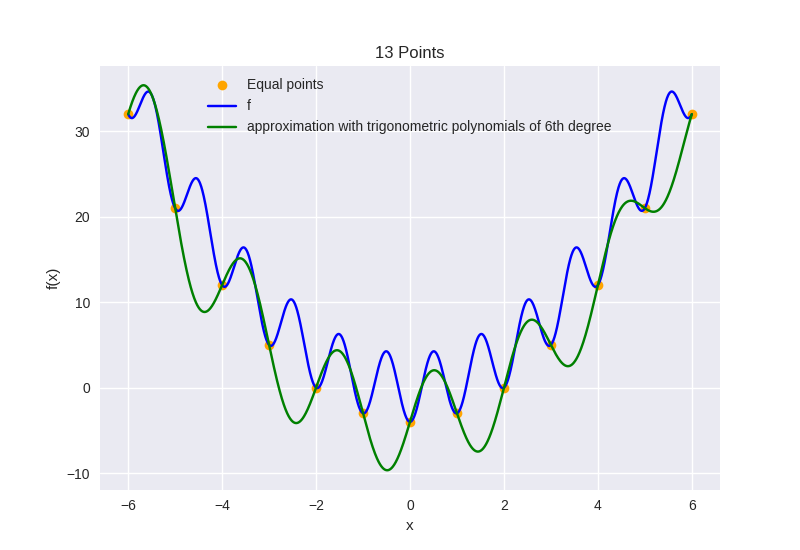
\includegraphics[width=0.9\textwidth]{img/tripoly_6_13.png}
    \caption{Aproksymacja średniokwadratowa wielomianami trygonometrycznymi 6 stopnia}
\end{figure}

\begin{figure}[H]
    \centering
    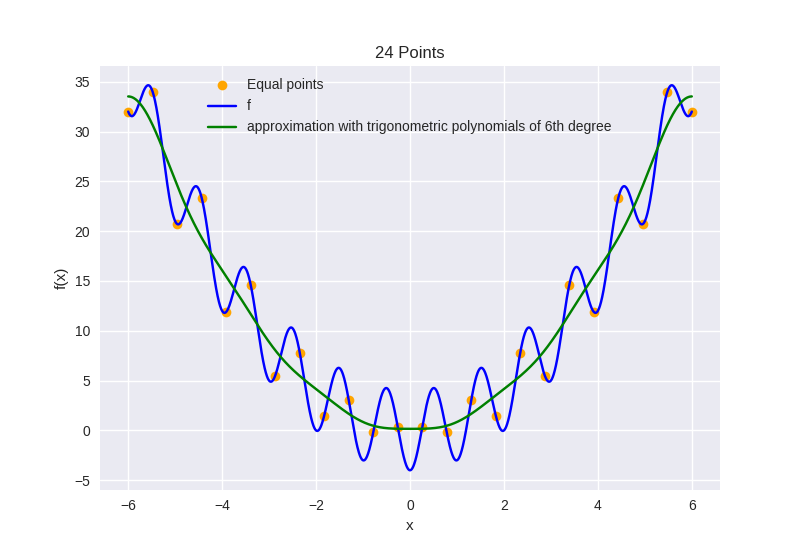
\includegraphics[width=0.9\textwidth]{img/tripoly_6_24.png}
    \caption{Aproksymacja średniokwadratowa wielomianami trygonometrycznymi 6 stopnia}
\end{figure}

Wielomiany szóstego stopnia dla mniejszych liczb węzłów bardziej przypominają wykres funkcji aproksymowanej, zawierają kilka
charakterystycznych "zębów", jednak ze wzrostem liczby punktów, wykres się wygładza, ponieważ stopień jest zbyt niski, żeby
wiernie odwzorować funkcję $f$.

Wielomiany wyższych stopni wykazują podobną tendencję: dla niewielkich liczb węzłów mają więcej głębokich minimów i wysokich maksimów,
częściowo pokazują charakterystyczny kształt funkcji $f$, jednak gdy liczba punktów względem stopnia wielomianu staje się zbyt duża,
wygładzają się, tak więc liczba węzłów nie poprawia drastycznie dokładności.

\begin{figure}[H]
    \centering
    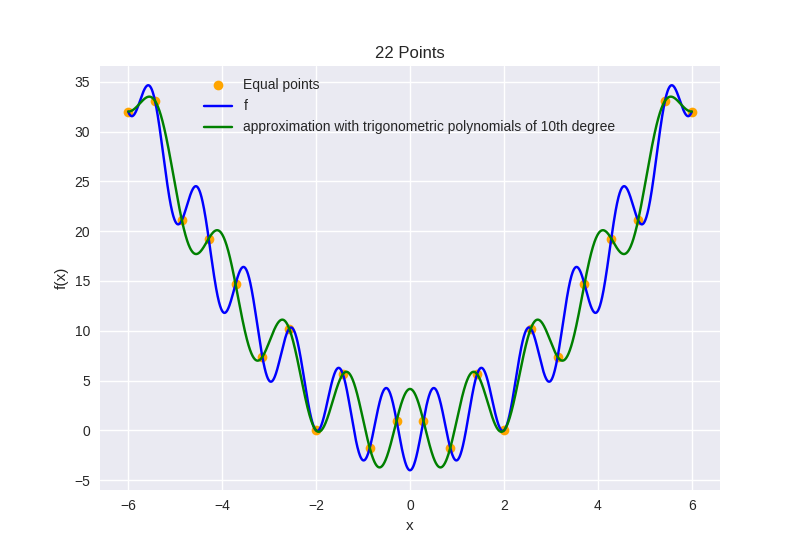
\includegraphics[width=\textwidth]{img/tripoly_10_22.png}
    \caption{Aproksymacja średniokwadratowa wielomianami trygonometrycznymi 10 stopnia}
\end{figure}

\begin{figure}[H]
    \centering
    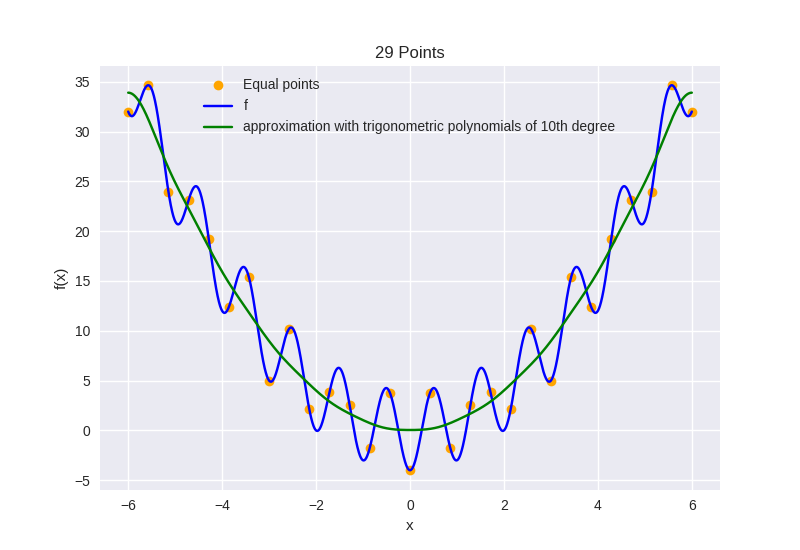
\includegraphics[width=\textwidth]{img/tripoly_10_29.png}
    \caption{Aproksymacja średniokwadratowa wielomianami trygonometrycznymi 10 stopnia}
\end{figure}

Najmniejszy stopień wielomianu, przy którym kształt funkcji jest dobrze odwzorowany, to dwanaście (jest to również liczba maksimów lokalnych funkcji $f$). 
Przy tej liczbie, dla najmniejszej poprawnej liczby węzłów, wykresy funkcji aproksymowanej i aproksymacyjnej pokrywają się w bardzo dużym stopniu, 
zwiększanie liczby węzłów nie daje natomiast dużej poprawy.

\begin{figure}[H]
    \centering
    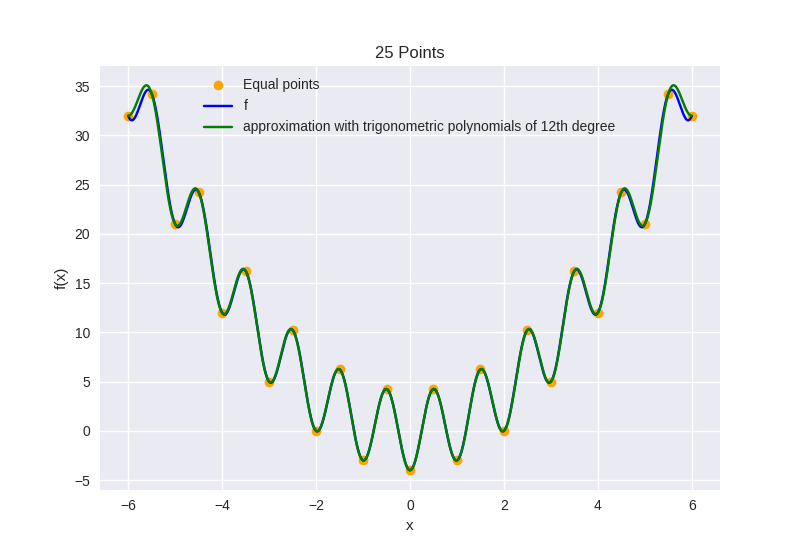
\includegraphics[width=0.9\textwidth]{img/tripoly_12_25.png}
    \caption{Aproksymacja średniokwadratowa wielomianami trygonometrycznymi 12 stopnia}
\end{figure}

\begin{figure}[H]
    \centering
    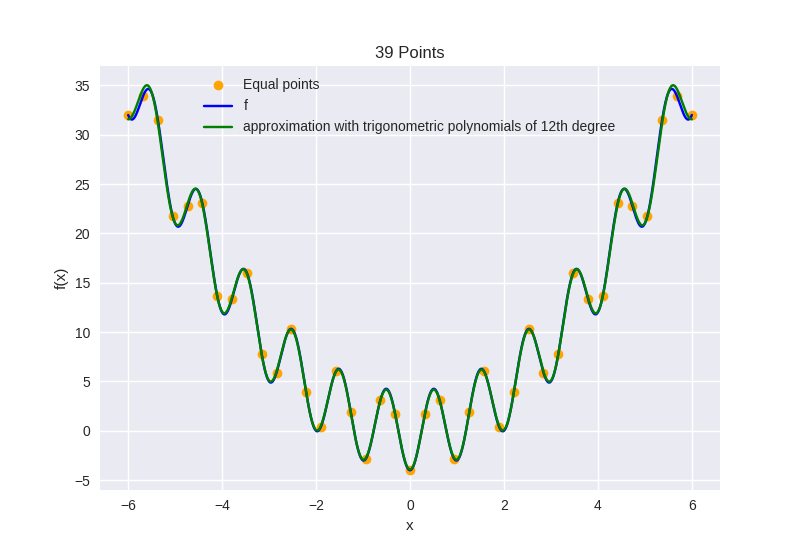
\includegraphics[width=0.9\textwidth]{img/tripoly_12_39.png}
    \caption{Aproksymacja średniokwadratowa wielomianami trygonometrycznymi 12 stopnia}
\end{figure}

Jak widać, zwiększanie liczby węzłów nie już zwiększa zbytnio dokładności. Poniżej wykres dla dwudziestego stopnia wielomianu,
jego dokładność nie zwiększyła się zbytnio w porównaniu do dwunastego stopnia (który był już bardzo dokładny).

\begin{figure}[H]
    \centering
    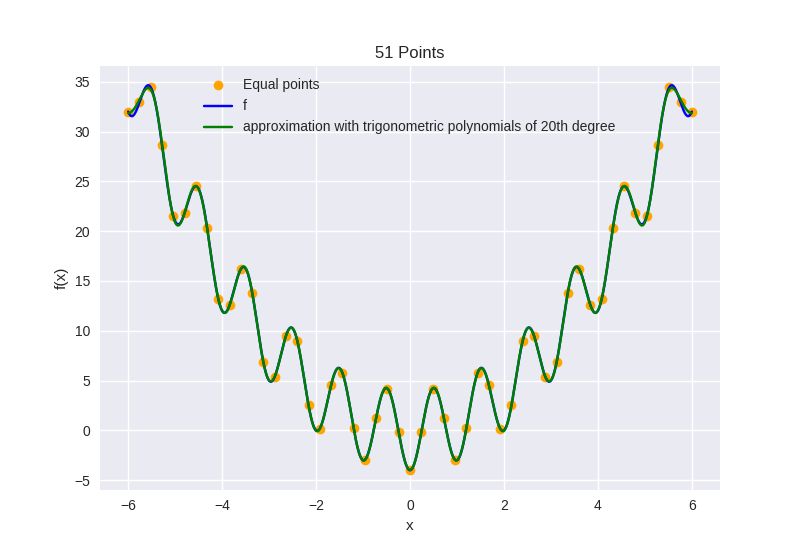
\includegraphics[width=\textwidth]{img/tripoly_20_51.png}
    \caption{Aproksymacja średniokwadratowa wielomianami trygonometrycznymi 20 stopnia}
\end{figure}

\subsection{Dokładności}
Pozostaje obliczenie dokładności oraz skonfrontowanie wyników z wnioskami uzyskanymi na podstawie analizy wykresów. Miarami dokładności będą:
\begin{itemize}
    \item
    średnia kwadratów odległości wartości wielomianu oraz funkcji $f$ dla 1000 równo oddalonych punktów,
    \item
    maksymalna odległość wartości wielomianu oraz funkcji $f$ dla 1000 równo oddalonych punktów.
\end{itemize}

\begin{table}[H]
\begin{adjustwidth}{-.7in}{-.7in} 
\begin{tabular}{|l|l|l|l|l|l|l|l|l|l|l|l|l|l|l|l|l|l|l|l|}
\hline
W\textbackslash{}S & 3 & 4 & 5 & 6 & 7 & 8 & 9 & 10 & 11 & 12 & ... & 20 \\ \hline
7 & 60.35 & X & X & X & X & X & X & X & X & X & ... & X \\ \hline
8 & 14.25 & X & X & X & X & X & X & X & X & X & ... & X \\ \hline
9 & 8.80 & 38.04 & X & X & X & X & X & X & X & X & ... & X \\ \hline
10 & 13.85 & 14.16 & X & X & X & X & X & X & X & X & ... & X \\ \hline
11 & 14.32 & 14.49 & 580.48 & X & X & X & X & X & X & X & ... & X \\ \hline
12 & 14.49 & 14.60 & 14.83 & X & X & X & X & X & X & X & ... & X \\ \hline
13 & 22.58 & 22.63 & 22.80 & 39.86 & X & X & X & X & X & X & ... & X \\ \hline
14 & 14.64 & 14.65 & 14.79 & 14.96 & X & X & X & X & X & X & ... & X \\ \hline
15 & 14.68 & 14.67 & 14.77 & 14.91 & 222.70 & X & X & X & X & X & ... & X \\ \hline
16 & 14.72 & 14.68 & 14.77 & 14.88 & 15.00 & X & X & X & X & X & ... & X \\ \hline
17 & 8.42 & 14.70 & 14.76 & 14.86 & 14.96 & 39.35 & X & X & X & X & ... & X \\ \hline
18 & 8.41 & 7.97 & 14.76 & 14.85 & 14.93 & 15.02 & X & X & X & X & ... & X \\ \hline
19 & 8.41 & 7.97 & 7.80 & 14.84 & 14.92 & 14.99 & 32.07 & X & X & X & ... & X \\ \hline
20 & 8.40 & 7.97 & 7.80 & 7.72 & 14.90 & 14.97 & 15.04 & X & X & X & ... & X \\ \hline
21 & 8.40 & 7.97 & 7.80 & 7.72 & 7.68 & 14.96 & 15.02 & 17.24 & X & X & ... & X \\ \hline
22 & 8.40 & 7.97 & 7.80 & 7.72 & 7.68 & 7.66 & 15.00 & 15.05 & X & X & ... & X \\ \hline
23 & 8.40 & 7.97 & 7.80 & 7.72 & 7.68 & 7.66 & 7.65 & 15.04 & 15.07 & X & ... & X \\ \hline
24 & 8.39 & 7.97 & 7.80 & 7.72 & 7.68 & 7.66 & 7.65 & 7.64 & 15.06 & X & ... & X \\ \hline
25 & 8.39 & 7.97 & 7.80 & 7.72 & 7.68 & 7.66 & 7.65 & 7.64 & 7.64 & 0.077 & ... & X \\ \hline
26 & 8.39 & 7.97 & 7.80 & 7.72 & 7.68 & 7.66 & 7.65 & 7.64 & 7.64 & 0.074 & ... & X \\ \hline
27 & 8.39 & 7.97 & 7.80 & 7.72 & 7.68 & 7.66 & 7.65 & 7.65 & 7.64 & 0.069 & ... & X \\ \hline
28 & 8.39 & 7.97 & 7.80 & 7.72 & 7.68 & 7.66 & 7.65 & 7.65 & 7.64 & 0.064 & ... & X \\ \hline
29 & 8.39 & 7.97 & 7.80 & 7.72 & 7.68 & 7.66 & 7.65 & 7.65 & 7.64 & 0.060 & ... & X \\ \hline
30 & 8.39 & 7.97 & 7.80 & 7.72 & 7.68 & 7.66 & 7.65 & 7.65 & 7.64 & 0.057 & ... & X \\ \hline
31 & 8.39 & 7.97 & 7.80 & 7.72 & 7.68 & 7.66 & 7.65 & 7.65 & 7.64 & 0.054 & ... & X \\ \hline
32 & 8.39 & 7.97 & 7.80 & 7.72 & 7.68 & 7.66 & 7.65 & 7.65 & 7.64 & 0.051 & ... & X \\ \hline
33 & 8.39 & 7.97 & 7.80 & 7.72 & 7.68 & 7.66 & 7.65 & 7.65 & 7.64 & 0.049 & ... & X \\ \hline
34 & 8.39 & 7.97 & 7.80 & 7.72 & 7.68 & 7.66 & 7.65 & 7.65 & 7.64 & 0.047 & ... & X \\ \hline
35 & 8.39 & 7.97 & 7.80 & 7.72 & 7.68 & 7.66 & 7.65 & 7.65 & 7.64 & 0.045 & ... & X \\ \hline
36 & 8.38 & 7.97 & 7.80 & 7.72 & 7.68 & 7.66 & 7.65 & 7.64 & 7.64 & 0.044 & ... & X \\ \hline
37 & 8.38 & 7.97 & 7.80 & 7.72 & 7.68 & 7.66 & 7.65 & 7.64 & 7.64 & 0.042 & ... & X \\ \hline
38 & 8.38 & 7.97 & 7.80 & 7.72 & 7.68 & 7.66 & 7.65 & 7.64 & 7.64 & 0.041 & ... & X \\ \hline
39 & 8.38 & 7.97 & 7.80 & 7.72 & 7.68 & 7.66 & 7.65 & 7.64 & 7.64 & 0.040 & ... & X \\ \hline
40 & 8.38 & 7.97 & 7.80 & 7.72 & 7.68 & 7.66 & 7.65 & 7.64 & 7.64 & 0.039 & ... & X \\ \hline
41 & 8.38 & 7.97 & 7.80 & 7.72 & 7.68 & 7.66 & 7.65 & 7.64 & 7.64 & 0.038 & ... & 452.961 \\ \hline
42 & 8.38 & 7.97 & 7.80 & 7.72 & 7.68 & 7.66 & 7.65 & 7.64 & 7.64 & 0.037 & ... & 0.017 \\ \hline
43 & 8.38 & 7.97 & 7.80 & 7.72 & 7.68 & 7.66 & 7.65 & 7.64 & 7.64 & 0.036 & ... & 0.016 \\ \hline
44 & 8.38 & 7.97 & 7.80 & 7.72 & 7.68 & 7.66 & 7.65 & 7.64 & 7.64 & 0.035 & ... & 0.015 \\ \hline
45 & 8.38 & 7.97 & 7.80 & 7.72 & 7.68 & 7.66 & 7.65 & 7.64 & 7.64 & 0.034 & ... & 0.015 \\ \hline
46 & 8.38 & 7.97 & 7.80 & 7.72 & 7.68 & 7.66 & 7.65 & 7.64 & 7.64 & 0.034 & ... & 0.014 \\ \hline
47 & 8.38 & 7.97 & 7.80 & 7.72 & 7.68 & 7.66 & 7.65 & 7.64 & 7.64 & 0.033 & ... & 0.014 \\ \hline
48 & 8.38 & 7.97 & 7.80 & 7.72 & 7.68 & 7.66 & 7.65 & 7.64 & 7.64 & 0.032 & ... & 0.013 \\ \hline
\end{tabular}
\end{adjustwidth}
\caption{Średnie kwadratów odległości (rzędy - węzły, kolumny - stopnie)}
\end{table}

\begin{table}[H]
\begin{adjustwidth}{-.6in}{-.6in} 
\begin{tabular}{|l|l|l|l|l|l|l|l|l|l|l|l|l|l|l|l|l|l|l|l|}
\hline
W\textbackslash{}S & 3 & 4 & 5 & 6 & 7 & 8 & 9 & 10 & 11 & 12 & ... & 20 \\ \hline
7 & 16.04 & X & X & X & X & X & X & X & X & X & ... & X \\ \hline
8 & 8.38 & X & X & X & X & X & X & X & X & X & ... & X \\ \hline
9 & 6.22 & 14.10 & X & X & X & X & X & X & X & X & ... & X \\ \hline
10 & 7.29 & 8.86 & X & X & X & X & X & X & X & X & ... & X \\ \hline
11 & 8.11 & 8.71 & 42.32 & X & X & X & X & X & X & X & ... & X \\ \hline
12 & 7.75 & 8.69 & 8.05 & X & X & X & X & X & X & X & ... & X \\ \hline
13 & 9.35 & 8.63 & 9.09 & 14.88 & X & X & X & X & X & X & ... & X \\ \hline
14 & 7.74 & 8.61 & 7.94 & 8.42 & X & X & X & X & X & X & ... & X \\ \hline
15 & 8.01 & 8.51 & 8.47 & 7.64 & 28.04 & X & X & X & X & X & ... & X \\ \hline
16 & 7.59 & 8.57 & 7.57 & 8.35 & 8.60 & X & X & X & X & X & ... & X \\ \hline
17 & 5.73 & 7.56 & 6.63 & 6.51 & 6.71 & 13.38 & X & X & X & X & ... & X \\ \hline
18 & 5.70 & 5.07 & 8.07 & 8.31 & 8.02 & 8.28 & X & X & X & X & ... & X \\ \hline
19 & 5.68 & 5.06 & 4.48 & 7.94 & 8.18 & 8.22 & 14.06 & X & X & X & ... & X \\ \hline
20 & 5.66 & 5.05 & 4.49 & 4.39 & 7.75 & 8.21 & 8.15 & X & X & X & ... & X \\ \hline
21 & 5.64 & 5.04 & 4.49 & 4.38 & 4.22 & 7.85 & 8.08 & 10.17 & X & X & ... & X \\ \hline
22 & 5.63 & 5.04 & 4.49 & 4.38 & 4.21 & 4.14 & 7.84 & 8.16 & X & X & ... & X \\ \hline
23 & 5.62 & 5.03 & 4.49 & 4.37 & 4.21 & 4.14 & 4.08 & 7.85 & 8.08 & X & ... & X \\ \hline
24 & 5.61 & 5.03 & 4.49 & 4.37 & 4.20 & 4.13 & 4.08 & 4.05 & 7.86 & X & ... & X \\ \hline
25 & 5.60 & 5.02 & 4.49 & 4.36 & 4.20 & 4.13 & 4.07 & 4.05 & 3.96 & 1.138 & ... & X \\ \hline
26 & 5.59 & 5.02 & 4.49 & 4.36 & 4.20 & 4.12 & 4.07 & 4.04 & 3.96 & 1.095 & ... & X \\ \hline
27 & 5.58 & 5.02 & 4.49 & 4.36 & 4.19 & 4.12 & 4.07 & 4.04 & 3.97 & 1.062 & ... & X \\ \hline
28 & 5.57 & 5.01 & 4.49 & 4.36 & 4.19 & 4.12 & 4.07 & 4.04 & 3.97 & 1.033 & ... & X \\ \hline
29 & 5.56 & 5.01 & 4.49 & 4.36 & 4.19 & 4.12 & 4.07 & 4.04 & 3.97 & 1.006 & ... & X \\ \hline
30 & 5.56 & 5.01 & 4.49 & 4.35 & 4.19 & 4.12 & 4.06 & 4.04 & 3.97 & 0.981 & ... & X \\ \hline
31 & 5.55 & 5.01 & 4.49 & 4.35 & 4.19 & 4.12 & 4.06 & 4.03 & 3.97 & 0.958 & ... & X \\ \hline
32 & 5.55 & 5.01 & 4.49 & 4.35 & 4.19 & 4.12 & 4.06 & 4.03 & 3.97 & 0.938 & ... & X \\ \hline
33 & 5.54 & 5.00 & 4.49 & 4.35 & 4.19 & 4.11 & 4.06 & 4.03 & 3.97 & 0.919 & ... & X \\ \hline
34 & 5.54 & 5.00 & 4.49 & 4.35 & 4.19 & 4.11 & 4.06 & 4.03 & 3.98 & 0.901 & ... & X \\ \hline
35 & 5.54 & 5.00 & 4.49 & 4.35 & 4.19 & 4.11 & 4.06 & 4.03 & 3.98 & 0.884 & ... & X \\ \hline
36 & 5.53 & 5.00 & 4.49 & 4.35 & 4.19 & 4.11 & 4.06 & 4.03 & 3.98 & 0.868 & ... & X \\ \hline
37 & 5.53 & 5.00 & 4.49 & 4.35 & 4.19 & 4.11 & 4.06 & 4.03 & 3.98 & 0.854 & ... & X \\ \hline
38 & 5.52 & 5.00 & 4.49 & 4.35 & 4.19 & 4.11 & 4.06 & 4.03 & 3.98 & 0.841 & ... & X \\ \hline
39 & 5.52 & 5.00 & 4.49 & 4.35 & 4.19 & 4.11 & 4.06 & 4.03 & 3.98 & 0.828 & ... & X \\ \hline
40 & 5.52 & 5.00 & 4.49 & 4.35 & 4.19 & 4.11 & 4.06 & 4.03 & 3.98 & 0.816 & ... & X \\ \hline
41 & 5.52 & 5.00 & 4.49 & 4.35 & 4.19 & 4.11 & 4.06 & 4.03 & 3.98 & 0.805 & ... & 30.721 \\ \hline
42 & 5.51 & 5.00 & 4.49 & 4.35 & 4.19 & 4.11 & 4.06 & 4.03 & 3.98 & 0.794 & ... & 0.667 \\ \hline
43 & 5.51 & 5.00 & 4.49 & 4.35 & 4.19 & 4.12 & 4.06 & 4.03 & 3.98 & 0.784 & ... & 0.655 \\ \hline
44 & 5.51 & 5.00 & 4.49 & 4.35 & 4.19 & 4.12 & 4.06 & 4.03 & 3.98 & 0.774 & ... & 0.643 \\ \hline
45 & 5.51 & 4.99 & 4.49 & 4.35 & 4.19 & 4.12 & 4.06 & 4.03 & 3.98 & 0.765 & ... & 0.632 \\ \hline
46 & 5.51 & 4.99 & 4.49 & 4.35 & 4.19 & 4.12 & 4.06 & 4.03 & 3.98 & 0.756 & ... & 0.621 \\ \hline
47 & 5.50 & 4.99 & 4.49 & 4.35 & 4.19 & 4.12 & 4.06 & 4.03 & 3.98 & 0.748 & ... & 0.611 \\ \hline
48 & 5.50 & 4.99 & 4.49 & 4.35 & 4.19 & 4.12 & 4.06 & 4.03 & 3.98 & 0.740 & ... & 0.602 \\ \hline
\end{tabular}
\end{adjustwidth}
\caption{Maksymalne odległości (rzędy - węzły, kolumny - stopnie)}
\end{table}

Z tabel wynika, że wzrost liczby węzłów ma wpływ na dokładność tylko do pewnego momentu, lub prawie nie ma wpływu dla stopni
wielomianu, które dobrze przybliżają funkcję $f$. Natomiast zwiększanie liczby funkcji bazowych (stopnia wielomianu) wpływa istotnie na
dokładność aż do momentu, kiedy dokładność jest bardzo duża. Warto też zauważyć, że dla stopni większych od dwunastu czasami
występuje zjawisko, gdzie wielomian danego stopnia ma bardzo zaniżoną dokładność dla minimalnej liczby węzłów.

\subsection{Porównanie z aproksymacją średniokwadratową wielomianami algebraicznymi}
Ze względu na naturę funkcji $f$ aproksymacja przy użyciu wielomianów trygonometrycznych skutkuje lepszą dokładnością niż aproksymacja
przy użyciu wielomianów algebraicznych oraz osiąga ją dla mniejszych liczb funkcji bazowych i węzłów. Na przykład, poniżej porównanie:
wielomiany algebraiczne dla 25 funkcji bazowych (24 stopnia), 25 węzłów oraz wielomiany trygonometryczne dla 25 funkcji bazowych 
(12 stopnia), 25 węzłów.

\begin{figure}[H]
    \centering
    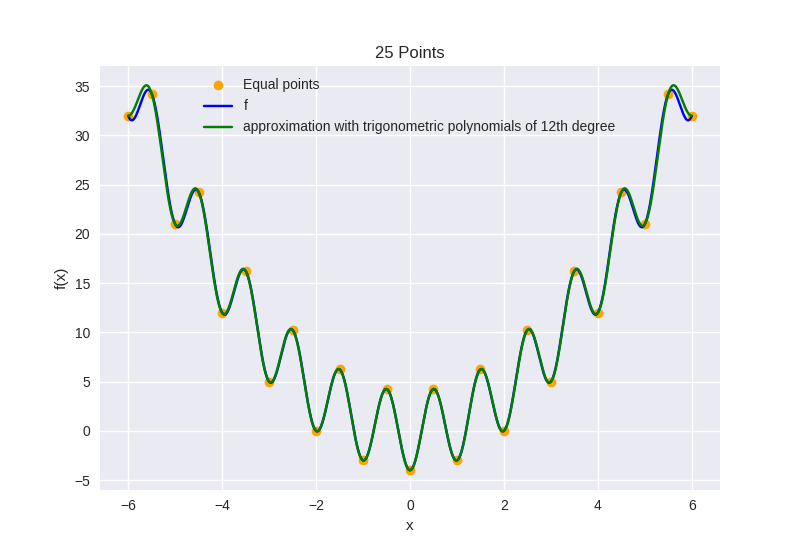
\includegraphics[width=\textwidth]{img/tripoly_12_25.png}
    \caption{Aproksymacja średniokwadratowa wielomianami trygonometrycznymi 12 stopnia}
\end{figure}

\begin{figure}[H]
    \centering
    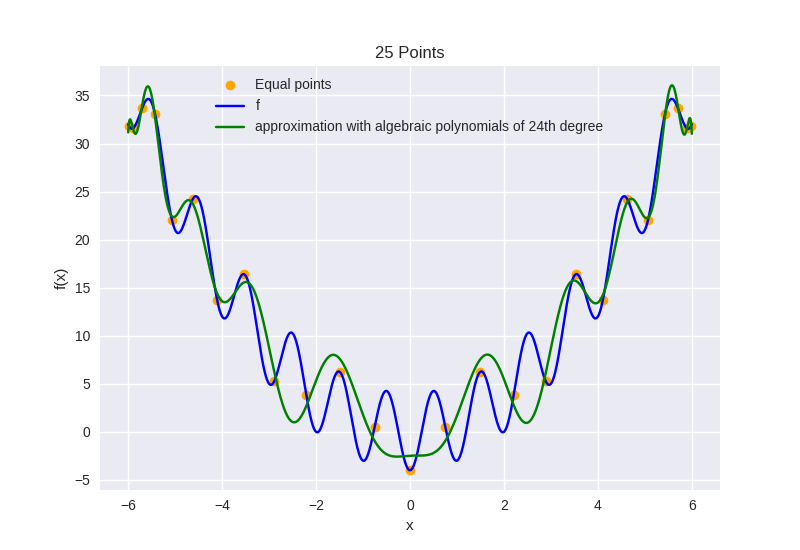
\includegraphics[width=\textwidth]{img/algpoly_24_25.png}
    \caption{Aproksymacja średniokwadratowa wielomianami algebraicznymi 24 stopnia}
\end{figure}

\section{Wnioski}
Aproksymacja średniokwadratowa wielomianami algebraicznymi jest skutecznym sposobem przybliżania funkcji, jeżeli nie musi być spełniony
warunek, że funkcja przybliżająca przechodzi przez dane punkty, lub punkty obarczone są błędami. Do aproksymacji można używać różnych liczb
wielomianów bazowych, użycie większej liczby wielomianów zazwyczaj skutkuje zwiększeniem dokładności, w przeciwieństwie
do zwiększania liczby węzłów. Dla pewnych funkji, jak ta przedstawiona tutaj, aproksymacja średniokwadratowa wielomianami 
trygonometrycznymi skutkje dużo lepszą dokładnością niż wielomianami algebraicznymi.

\end{document}